%%%%%%%%%%%%%%%%%%%%%%%%%%%%%%%%%%%%%%%%%%%%%%%%%%%%%%%%%%%%%%%%%%%%
%% I, the copyright holder of this work, release this work into the
%% public domain. This applies worldwide. In some countries this may
%% not be legally possible; if so: I grant anyone the right to use
%% this work for any purpose, without any conditions, unless such
%% conditions are required by law.
%%%%%%%%%%%%%%%%%%%%%%%%%%%%%%%%%%%%%%%%%%%%%%%%%%%%%%%%%%%%%%%%%%%%

\documentclass[
  printed, %% This option enables the default options for the
           %% digital version of a document. Replace with `printed`
           %% to enable the default options for the printed version
           %% of a document.
  table,   %% Causes the coloring of tables. Replace with `notable`
           %% to restore plain tables.
 oneside,
  lof,     %% Prints the List of Figures. Replace with `nolof` to
           %% hide the List of Figures.
  lot     %% Prints the List of Tables. Replace with `nolot` to
           %% hide the List of Tables.
  %% More options are listed in the user guide at
  %% <http://mirrors.ctan.org/macros/latex/contrib/fithesis/guide/mu/fi.pdf>.
]{fithesis3}
%% The following section sets up the locales used in the thesis.
\usepackage[resetfonts]{cmap} %% We need to load the T2A font encoding
\usepackage[T1,T2A]{fontenc}  %% to use the Cyrillic fonts with Russian texts.
\usepackage[
  main=slovak, %% By using `czech` or `slovak` as the main locale
                %% instead of `english`, you can typeset the thesis
                %% in either Czech or Slovak, respectively.
  english %% The additional keys allow
]{babel}        %% foreign texts to be typeset as follows:
%%
%%   \begin{otherlanguage}{german}  ... \end{otherlanguage}
%%   \begin{otherlanguage}{russian} ... \end{otherlanguage}
%%   \begin{otherlanguage}{czech}   ... \end{otherlanguage}
%%   \begin{otherlanguage}{slovak}  ... \end{otherlanguage}
%%
%% For non-Latin scripts, it may be necessary to load additional
%% fonts:
\usepackage{paratype}
\def\textrussian#1{{\usefont{T2A}{PTSerif-TLF}{m}{rm}#1}}
%%
%% The following section sets up the metadata of the thesis.
\thesissetup{
    date          = \the\year/\the\month/\the\day,
    university    = mu,
    faculty       = fi,
    type          = mgr,
    author        = Tomáš Márton,
    gender        = m,
    advisor       = RNDr. Daniel Tovarňák,
    title         = {Interaktivní správa a odhalování parsovacích pravidel pro logovací data},
    TeXtitle      = {Interaktivní správa a odhalování parsovacích pravidel pro logovací data},
    keywords      = {Logovanie, Clustering, Frequent Pattern Mining, Extended Nagappan-Vouk},
    TeXkeywords   = {Logovanie, Clustering, Frequent Pattern Mining, Extended Nagappan-Vouk},
    bib           = ./thesis.bib,
}
\thesislong{abstract}{
    Diplomová práca sa zaoberá odhaľovaním parsovacích vzorov systémových logov, konkrétne algoritmom Extended Nagappan-Vouk. Tento algoritmus vyhodnocuje a implementuje webové užíveteľské rozhranie pre tento algoritmus.
}
\thesislong{thanks}{
Rád by som poďakoval RNDr. Danielovi Tovarňakovi, vedúcemu tejto diplomovej práce, za vedenie a podnetné návrhy. Ďalej by som sa rád poďakoval svojej rodine a priateľom za podporu pri písaní tejto práce.
}
\usepackage{makeidx}      %% The `makeidx` package contains
\makeindex                %% helper commands for index typesetting.
%% These additional packages are used within the document:
\usepackage{paralist} %% Compact list environments
\usepackage{amsmath}  %% Mathematics
\usepackage{amsthm}
\usepackage{amsfonts}
\usepackage{url}      %% Hyperlinks
\usepackage{multirow} %% table multirow
\usepackage{array} %% table cell vertical centering
\usepackage{tabularx}
\usepackage{listings}
\usepackage{todonotes}
\usepackage{pgfplots}
\usetikzlibrary{calc}
\begin{document}

\chapter{Úvod}

Už od vynálezu počitačov produkuje každý softwér záznam o svojom behu. Tieto záznamy sa volajú logové súbory a slúžia programátorom a systémovým administrátorom na odladenie chýb programu a jeho monitorovanie. Logové súbory sú vytvárané programátormi vo forme viet hovorového jazyka, obsahujúcich všetky dôležité informácie o~udalosti v programe, ktorá práve nastala. Vo výsledku teda obsahujú jedinečné kvantum informácií, ktoré nie sú inak dostupné. Kvôli rozmachu technológií sa však rapídne zvýšil objem logovacích súborov, v ktorých už viac nie je možné triviálne nájsť požadované informácie. V praxi sa preto stretávame s prípadom, že síce máme data o udalostiach, ktoré nastali, ale nevieme ich nájsť a správne použiť, alebo ani nevieme, že tieto údaje máme. Sme teda bohatí na data, ale chudobní na informácie.
\par Z tohto dôvodu je nutné vedieť informácie o udalosti v programe z~logových súborov efektívne a automaticky extrahovať a predpripraviť na ďalšie spracovanie. To sa deje vytvorením parsovacích vzorov, ku~ktorým vieme každú udalosť jednoznačne priradiť. Momentálne však neexistuje nástroj, ktorý by takéto vzory vytvoril nad ľubovoľnou množinou vstupných logovacích súborov v dostatočnej kvalite. Existujúce algoritmy trpia na rôzne nedostatky, ako aj na potrebu detailného nastavenia vstupných parametrov.
\par V práci sa zaoberáme rozšírenou verziou algoritmu Nagappan-Vouk, vyvinutou vedúcim práce RNDr. Danielom Tovarňákom. Tento algoritmus slúži na odhaľovanie parsovacích vzorov v logovacích súboroch. Vychádza z algoritmov popísaných v práci, pričom odstra\-ňu\-je ich známe nedostatky za pridania jednoduchej užívateľskej interakcie. Cieľom tejto práce je teda naimplementovať užívateľské rozhranie, ktoré bude plne podporovať algoritmus Nagappan-Vouk, pokúsiť sa zlepšiť presnosť výsledných parsovacích vzorov a porovnať výsledky voči podobným algoritmom.
 \par Práca sa člení ....
\chapter{Problematika logovania}

Logové súbory sú neoddeliteľnou súčasťou každého softwéru. Či už sa jedná o operačný systém, aplikačný server, softwér v sieťových prvkoch alebo koncovú užívateľskú aplikáciu. 
\par Logové súbory zaznamenávajú všetky udalosti od štartu, cez beh a chybové stavy až po ukončenie aplikácie. Ich analýza je často jediným spôsobom, ako odhaliť chybu, lebo logovanie nijako nenarúša ani neovplyvňuje beh programu. To predstavuje presný opak analýzy bežiaceho programu, pri ktorej analytický proces priamo komunikuje s programom za časovo alebo zdrojovo kritických podmienok  \parencite{jvaldman}. Analýza logových súborov sa takisto môže využiť aj na detekciu anomálií, monitorovanie systému, odhadovanie a plánovanie záťaže systému \parencite{logengineering}.
\par Do logových súborov sú zapisované pološtrukturované správy, ktoré vývojári softwéru používajú kvôli jednoduchosti a flexibilite \parencite{he2016, ibm}. Informácie, ktoré sa zvyčajne nachádzajú v popise v každej logovacej správe \parencite{weblog, datapreprocessing, sshd}, sú:
\begin{itemize}
  \item dátum a čas
  \item ip adresa alebo hostname
  \item komponenta
  \item protokol
\end{itemize}
\par Vo všeobecnosti síce nie je ustálený jednotný formát správ, ale existujú dobre známe formáty ako napr. \emph{Common Log Format}, používaný pre logovanie http požiadavkov \parencite{CLF} , flexibilnejši \emph{Extended Log Format} \parencite{ELF} alebo \emph{Syslog format}, využívaný pre logovanie udalostí v systéme Unix \parencite{syslog}. Tieto formáty sú často využívané a existujú pre ne aj analytické nástroje. \

\section{Motivácia}

\par Hoci je zapisovanie a ukladanie logových súborov jednoduchá a lacná úloha, ich ďalšia analýza môže zabrať značné zdroje, čas aj sofistikované metódy. V extrémnych prípadoch môže jeden uzol vygenerovať až okolo pol milióna správ za deň, čo v sledovanom systéme vyústilo do 400 GB nekomprimovaných dát za 2 mesiace \parencite{google}. Aj keď sa odprostíme od takýchto prípadov, logovacie súbory sú stále príliš veľké na manuálne spracovanie, a preto je potrebné proces ich spracovania automatizovať. Počas tohto procesu extrahujeme z logovacej správy jej statickú a dynamickú časť. Statická časť predstavuje konštantný reťazec znakov a budeme ho ďalej nazývať parsovací vzor. Dynamickú časť tvoria parametre parsovacieho vzoru a môžu byť pre každú správu rôzne. Výsledok extrakcie môžeme vidieť v tabuľke \ref{tab:a}, kde je dynamická časť znázornená znakom \emph{*}. 

\begin{table}[htbp]
\centering
\begin{tabularx}{\textwidth}{X}
\multicolumn{1}{c}{Logové správy}                                                                 \\ \hline
Generating 768 bit RSA key                                     \\
Generating 2048 bit RSA key                                    \\
Illegal user admin from 218.49.183.17                          \\
Illegal user guest from 218.49.183.17                          \\
Failed password for test from 218.49.183.17 port 49266 ssh2    \\
Accepted password for test from 192.168.15.135 port 49266 ssh2 \\
Failed password for root from 218.49.183.17 port 1066 ssh2     \\
Accepted password for root from 192.168.20.185 port 1066 ssh2  \\
\multicolumn{1}{c}{\multirow{2}{*}{ $\Big\Downarrow$ }}                                                             \\
\multicolumn{1}{c}{}                                                                              \\
\multicolumn{1}{c}{Nájdené parsovacie vzory}                                                      \\ \hline
Generating * bit RSA key                                      \\
Illegal user * from *                                          \\
* password for * from * port * ssh2                           
\end{tabularx}
\caption{Logové správy z sshd a ich parsovacie vzory}
\label{tab:a}
\end{table}

\par Triviálny prístup je použiť jednoduchú sadu vzorov napísaných použitím regulárnych výrazov. Je to síce zlepšenie, ale bez špecifickej znalosti zdrojového kódu nie je možné odhaliť všetky vzory. Navyše sa ukázalo ako neudržateľné spravovať takéto vzory dlhodobo, kedže logovacie správy sa často menia \parencite{xu2010}. Preto je potrebné mať k dispozícií nástroj, ktorý vzory odhalí automaticky.









\chapter{Odhaľovanie parsovacích vzorov správ}

Odhaľovanie parsovacích vzorov sa z~rozšírením distibuovaných sytémov a cloudu a tým spojeného nárastu objemu logovacích správ stáva pomerne dobre študovaným problémom. Bolo vyvynutých mnoho algoritmov riešiacich daný problém, ale žiaden z~nich zatiaľ neponúka postačujúce riešenie. Medzi najčastejšie používané patria riešenia založené na analýze zdrojových kódov alebo na metóde clustrovania.

\section{Analýza zdrojových kódov}

Je to pomerne presná metóda, kde za pomoci statickej analýzy vieme vo väčšine prípadov odhaliť všetky parsovacie vzory.
Rôzne programovacie jazyky ale používajú rôzny štýl logovania. Programovací jazyk C napr. používa volanie funkcie \emph{printf}.
V~tomto prípade sa snažíme nájsť volania tejto funkcie a zároveň odvodiť typy parametrov.
Pre objektovo orientované jazyky je situácia trochu komplikovanejšia, ako môžeme vidieť na obr. \ref{fig:static}. Po~prvé, vo väčšine prípadov používajú nejakú logovaciu abstrakciu a jej rozhranie, ktoré musíme identifikovať. Po~druhé, v~objektovo orientovanom programovaní sa na výpis reprezentácie objektu používa metóda \emph{toString}, čo je aj dôvod, prečo sú nájdené parsovacie vzory neúplné a je nutné ďalej rekurzívne investigovať metódu \emph{toString} na všetkych parametroch nájdeného parsovacieho vzoru.

\begin{figure}[htbp]
\centering
\begin{minipage}{0.9\textwidth}
\lstset{tabsize=4,columns=flexible,breaklines=true,breakatwhitespace=true, showstringspaces=false}
\begin{lstlisting}
class Session {
	String uid;
	
	@Override
	public String toString() {
		return "session with uid=" + uid;
	}
}

if (logger.isDebugEnabled()) {
	logger.debug("Transport error in " + session);
}

2017-05-12 20:52:39 DEBUG SomeService:19 - Transport error in session with uid=92ebcb67fe33s
\end{lstlisting} 		
\end{minipage}
\caption{Logovacia správa a kód, ktorý ju spôsobil v~jazyku Java}
\label{fig:static} 
\end{figure}

Hlavným negatívom, ktorý vyplýva z~podstaty analýzy zdrojových kódov, je značné množstvo času potrebné na správne identifikovanie parsovacích vzorov. Túto analýzu musíme vykonať pre každú novú verziu zdrojových kódov, čo ďalej zvyšuje zložitosť. Podmienkou u~tejto metódy je aj potreba mať prístup k~zdrojovým kódom, čo nie je vždy možné. 

\section{ Metóda clustrovania}
Pre potreby definície clustrovania logovacích správ si zadefinujme logovaciu správu ako bod definovaný n-početnou množinou nominálnych atribútov. Potom clustrovanie vieme popísať ako hľadanie rozdelenia takýchto bodov do konečnej skupiny kategórií -- clustrov, kde body v~jednom clustri sú si navzájom podobné, a zároveň čo najviac rozdielne od členov iných clustrov na základe svojich atribútov \parencite{iplom}. Na určenie toho, ako veľmi sú dve správy podobné, sa používa vzdialenostná funkcia. Ako bolo spomenuté v \parencite{logcluster}, vzdialenostné funkcie tradičných clustrovacích algoritmov vyžadujú tieto vlastnosti: 

\begin{enumerate}
  \item tokeny prevažne numerického tvaru
  \item fixný a nízky počet tokenov
  \item možnosť ignorovať poradie
  \item atribúty prevažne numerického tvaru 
  \item fixný a nízky počet atribútov 
\end{enumerate}

Tieto vlastnosti ale body reprezentujúce logovacie správy nespĺňajú. Je to spôsobené tým, že body s nominálnymi atribútmi mávajú často variabilný počet atribútov. Preto nie je triviálne určiť, ako sa bude vzdialenosť týchto bodov merať, aj keď existujú vzdialenostné funkcie pre body s nominálnymi atribútmi, napr. Jaccardov koeficient \parencite{slct}. Ďalej v \parencite{logcluster} bolo ukázané, že doterajšie vzdialenostné funkcie nepracujú presne v pri počte atribútov vyššom ako 10 a často neodhalia cluster. Kombinácia týchto vlastností spôsobuje, že tradičné vzdialenostné funkcie sú na clustrovanie logovacích správ nevhodné. Spôsobov, podľa ktorých možno jednotlivé clustre vytvárať, je niekoľko a každý algoritmus používa svoj postup, ako si ukážeme ďalej. Najprv si ale pre nasledujúcu časť zadefinujeme pojmy, ktoré budeme používať pri popise algoritmov. Logovací súbor budeme nazývať dataset, jeho jednotlivé riadky budeme považovať za správy, ktorých každé slovo bude reprezentovať jeden token. Ďalej kvôli všeobecne zaužívanej konvencii budeme dynamickú časť nájdeného parsovacieho vzoru označovať ako wildcard a v~samotnom vzore ho budeme nahradzovať znakom \emph{*}. 


\subsection{SLCT - Simple Logfile Clustering Tool}
Tvorca SLCT \parencite{slct, slctloghound} si všíma 2 kľúčové vlastnosti logovacích súborov, o~ktoré sa opieral pri tvorbe algoritmu. Prvá vlastnosť je, že väčšina slov sa v~datasete nevyskytuje často a nezanedbateľná časť dokonca len raz. Druhá vlastnosť hovorí, že medzi slovami, ktoré sa vyskytujú často, je silná korelácia. Neformálne povedané, často sa vyskytujúce slová tvoria statickú časť a zvyšné slova dynamickú časť logovacej správy. Algoritmus na vstupe očakáva hraničnú hodnotu N, podľa ktorej určí, či bude dané slovo považované za statickú alebo dynamickú časť.  SLCT pracuje v~nasledujúcich troch krokoch.

\begin{enumerate}
  \item Všetky správy v~datasete rozloží na dvojice \emph{(pozícia, token)} a spočíta počet výskytov danej dvojice v~datasete. Pre rozklad správy na tokeny sa používa ako delimiter znak medzery. Ak výskyt dvojice prekračuje hraničnú hodnotu N, dvojicu nazývame frekventovaná. Napr. \emph{(1, Generating)}.
  \item Pre každú správu v~datasete vezme algoritmus všetky frekventované dvojice, ktoré potom spolu tvoria kandidátnu množinu, napr. \emph{{(1,Generating), (3,bit), (4,RSA), (5, key)}}. 
  \item Ak sa kandidátna množina nachádza v~logovacom súbore častejšie ako hraničná hodnota N, potom je zvolený cluster. Cluster je vytvorený doplnením wildcard za chýbajúce pozície v~riadku, takže vysledný pattern vyzerá takto \emph{Generating * bit RSA key}.
\end{enumerate}

Riadky, ktoré nepatria k~žiadnemu clustru, tvoria špeciálny cluster nazývaný outliers. Všimnime si, že algoritmus vôbec nezaznamenáva pozície medzier ani počet tokenov v~pôvodnej správe. Preto kvôli spôsobu, akým tvorí clustre, SLCT nevie odhaliť wildcard na konci riadku. Vezmime si kandidátnu množinu $\{(1,Illegal), (2,user), (4,from)\} $. SLCT vytvorí pattern \emph{Illegal user * from}. Správny pattern by mal vyzerať takto  \emph{Illegal user * from *}.

\subsection{Naggapan-Vouk algoritmus}
Kľúčová vlastnosť, na ktorej Naggapan a Vouk postavili ich algoritmus \parencite{nagappanvouk}, je skutočnosť, že keď sa konkrétny pattern nachádza v~datasete na viacerých miestach z~rôznymi parametrami, jeho statická časť sa bude vyskytovať vo väčšine prípadov, zatiaľ čo dynamická časť len pár krát. Preto Nagappan-Vouk buduje tabuľku frekvencií, ako vidíme v tab. \ref{fig:naggapan}. Priebeh algoritmu:

\begin{enumerate}
  \item Vybudujeme si frekvenčnú tabuľku, ktorá obsahuje informáciu, koľko krát sa dané slovo nachádza na konkrétnej pozícií v~datasete. Neformálne povedané, riadky sú tokeny a stĺpce sú pozície, na ktorých sa token nachádza.
  \item Pre každú správu si vo frekvenčnej tabuľke vyhľadáme frekvencie všetkých tokenov správy. Nájdeme frekvenciu, ktorá sa vyskytuje najčastejšie. V~prípade, že takýchto frekvencií je viac, použijeme nižšiu frekvenciu.
  \item Každý token, ktorý má frekvenciu vyššiu alebo rovnú ako frekvencia nájdená v~minulom kroku, je označený ako statická časť. Zvyšné slová sú analogicky dynamická časť.
\end{enumerate}

\begin{table}[htbp]
\centering
\begin{tabularx}{175px}{ | X | c | c | c | c | c | }
\hline
           & 1 & 2 & 3 & 4 & 5 \\ \hline
768        & 0 & 1 & 0 & 0 & 0 \\ \hline
2048       & 0 & 1 & 0 & 0 & 0 \\ \hline
bit        & 0 & 0 & 2 & 0 & 0 \\ \hline
Generating & 2 & 0 & 0 & 0 & 0 \\ \hline
key        & 0 & 0 & 0 & 0 & 2 \\ \hline
RSA        & 0 & 0 & 0 & 2 & 0 \\ \hline
\end{tabularx}
\caption{Frekvenčná tabuľka pre algoritmus Nagappan-Vouk}
\label{fig:naggapan}
\end{table}

Algoritmus Nagappan-Vouk odhalí aj wildcard na poslednej pozícií, ale generuje prekývajúce sa clustre a v~prípade málo frekventovaných správ neodhalí daný vzor. Algoritmus nepodporuje žiadnu formu vstupných parametrov, ktorá by zlepšila výsledky.

\subsection{IPLoM - Iterative partitioning log mining}
Algoritmus IPLoM \parencite{iplom}  funguje odlišne od algoritmov popísaných vyššie. Pracuje na princípe hierarchického rozdeľovania logových správ na segmenty, kde na konci algoritmu listy v~tejto hierarchickej štruktúre sú clustre, z~ktorých budú vytvorené parsovacie patterny. Algoritmus pracuje takto:

\begin{enumerate}
  \item Rozdelenie podľa počtu tokenov. Vychádza z~predpokladu, že každá správa, ktorá bola vygenerovaná rovnakým patternom, bude mať rovnakú dĺžku. Každý segment teda obsahuje n-tice, kde n je počet tokenov v~každej správe.
  \item Rozdelenie podľa pozície tokenu. Pre každý segment nájdeme pozíciu tokenu, na ktorej segment obsahuje najmenej unikátnych hodnôt naprieč všetkými správami. Segment ďalej rozdelíme podľa hodnôt na nájdenej pozícii.
  \item Rozdelenie podľa hľadania bijekcie. Pred samotným hľadaním bijekcie sú zo segmentu najskôr odčlenené správy, ktoré podľa heuristiky \emph{cluster goodness treshold} už formujú dobrý cluster. Pre zvyšné správy nájdeme 2 rôzne pozície tokenov, ktoré obsahujú najviac unikátnych hodnôt. Hľadáme bijekciu medzi množinami tokenov na týchto 2 pozíciách. Ak bijekcia existuje, správy sú odčlenené do novej časti. Ak miesto bijekcie existuje vzťah \emph{1-N} alebo \emph{N-1}, použijeme heuristiku \emph{lower and upper treshold}. V~prípade vzťahu \emph{N-M} sú buď ignorované alebo ďalej rozdelené na vzťahy \emph{1-N}.
  \item Formovanie clustrov. Každý finálny segment reprezentuje cluster. Pattern získame tak, že pozície tokenov s~kardinalitou unikátnych hodnôt rovnou 1 považujeme za statickú časť a zvyšné pozície za dynamickú časť patternu.
\end{enumerate}

IPLom bol navrhnutý tak, aby našiel všetky parsovacie vzory v~prvotnom behu bez nutnosti špecifikovať vstupné nastavenia. V~skutočnosti ale podporuje 4 nastavenia, ktorými môžme obmedziť počet nájdených vzorov ako aj ich granularitu \parencite{nagappanvouk}.

\subsection{Logcluster}

Logcluster je algoritmus, ktorý má vyriešiť známe nedostatky SLCT \parencite{logcluster}. Rovnako ako SLCT si všíma výskyt frekventovaných slov v~správach, ale na~rozdiel od SLCT neberie do úvahy ich pozíciu. Vďaka tomu vie algoritmus priradiť do jedného clustru aj správy, ktoré nemajú rovnaký počet tokenov. Logcluster vezme vstupný parameter \emph{s}  a rozdelí správy do clustrov tak, aby v~každom bolo aspoň \emph{s} správ. Ak je hodnota parametru \emph{s} určená zle, algoritmus produkuje buď príliš špecifické alebo príliš všeobecné parsovacie vzory. Autori preto dávajú odporúčanie, ako tento parameter správne nastaviť. Algoritmus podporuje prácu s~viacerými oddelovačmi slov, čo je v~praktickom použití veľmi potrebné a považujeme to za veľkú výhodu \parencite{logclustertool}. Pre ešte lepšie výsledky algoritmus používa heuristiky \emph{aggregate \, support} a \emph{join cluster}. Vysledné parsovacie vzory používajú pre wildcard zápis v~tvare \emph{*\{m,n\}}, napr. \emph{Generating *\{1,1\} bit RSA key}. Tento zápis označuje \emph{m} až \emph{n} tokenov oddelených delimitrom.


\subsection{Nedostatky}
Všetky vyššie zmienené algoritmy -- SLCT, Nagappan-Vouk a IPLoM, sú založené na pozícií tokenu v~správe. Z~toho vyplýva, že nie sú schopné detegovať dynamickú časť parsovacieho vzoru, ktorá by sa skladala z~viacerých tokenov. Ďalším nedostatkom týchto algoritmov je prekrývanie výsledných clustrov, ktoré by sa dalo odstrániť dodatočnou úpravou a spojením prekrývajúcich sa parsovacích vzorov. Logcluster tieto nedostatky síce nemá, ale správne nastavenie jeho heuristík môže byť náročná úloha.
\chapter{Rekurzívne clustrovanie pod dohľadom užívateľa}

Všetky algoritmy zmienené v~predchádzajúcej kapitole pomerne dobre odhaľujú parsovacie vzory, ktoré sa v~danom datasete objavujú často, a ich výsledky sú presné. Aby sme ale dosiahli odhalenie všetkých parsovacích vzorov pri zachovaní vysokej presnosti, musíme sa vysporiadať s~obmedzeniami clustrovacích algoritmov \parencite{Tovarnak2017}.

\subsection*{Rozdelenie správy na tokeny}
Prvým krokom všetkých prezentovaných algoritmov je rozdeliť parsovaciu správu na tokeny. V~tomto smere je potrebná väčšia variabilita pri~zadávaní oddeľovača slov. Nie všetky algoritmy totiž podporujú možnosť zadať aj iný oddeľovač ako medzera, ale ani podpora via\-cerých oddeľovačov tokenov nie je dostačujúca, ako si ukážeme na~príklade. \\

\indent \emph{Starting server with param timeout=2000 ms} \\
\indent \emph{Processing request 127.0.0.1/api/patterns?page-size=10\&page=3} \\

V~prvom prípade chceme použiť ako delimiter aj znak \emph{=} . V~druhom prípade je žiadúce, aby celá url adresa bola zachytená ako jeden para\-meter. Delimiter \emph{=} teda použiť nechceme, a preto by možnosť použiť iný delimiter pre rôzne logovacie správy pomohla ďalej spresniť výsledné parsovacie vzory.

\subsection*{Vstupné parametre}
Hodnota vstupných parametrov je vo vačšine prípadov jedným z~hlav\-ných faktorov, ktorý ovplyvňuje kvalitu výsledných parsovacích vzorov.
Pre~tieto hodnoty existujú odporúčania, ale najpresnejší výsledok získame až po manuálnej analýze datasetu, kde užívateľ po prezre\-tí správ datasetu spustí párkrát daný algoritmus a pokúsi sa nájsť parametre, pre ktoré budú výsledné parsovacie vzory čo najpresnej\-šie.

\subsection*{Kontrola výsledných parsovacích vzorov}
V~závislosti od vyššie zmienených nastavení dostaneme parsovacie vzory, ktoré buď zodpovedajú našej predstave, alebo nie. Komplikovanejšia situácia nasáva v~prípade, ak neexistuje všeobecné nastavenie algoritmu, ktoré by vrátilo všetky parsovacie vzory v~potrebnej kvalite. Tento problém sa dá obísť užívateľským rozdelením datasetu na menšie časti a na každú časť pustiť algoritmus s~vlastným nastavením. Toto je ale komplikované, zdĺhavé, náchylne k~chybám a~v~ne\-poslednom rade aj užívateľsky neprívetivé.

\section{RURC -- Recursive User-Reviewed Clustering}
\label{sec:rurc}
Z~hore uvedeného rozboru vyplýva, že ideálny algoritmus by mal zahŕňať určitý stupeň užívateľskej interakcie a mal by vedieť pracovať aj nad vybranou podmnožinou daného datasetu.
\par Vedúci práce, RNDr. Daniel Tovarňák, preto v~\parencite{Tovarnak2017} navrhol syste\-matický postup nazvaný \emph{Recursive User-Reviewed Clustering} znázornený na obr. \ref{fig:rurc}. Výsledkom je proces, pri ktorom užívateľ rekurzívne spúšťa algoritmus nad datasetom, pričom v~každom priebehu má možnosť potvrdiť finálne parsovacie vzory a odfiltrovať z~datasetu správy, ktoré k~nim patria.
\par Tento proces prebieha v~nasledujúcich krokoch:

\begin{enumerate}
  \item Odstránenie správ z~datasetu, ktoré prislúchajú k~už odhaleným parsovacím vzorom.
  \item Úvodný beh algoritmu s~defaultnými parametrami.
  \item Užívateľ rozhodne, ktoré parsovacie vzory sú akceptovateľné, a~tým zároveň z~datasetu odstráni príslušné správy.
  \item Užívateľ buď:
  	\begin{enumerate}
   		 \item spustí algoritmus nad celým datasetom so zmenenými parametrami a pokračuje od bodu 3.
   		 \item označí množinu vzorov, ktoré nie sú vhodné, spustí algoritmus nad podmnožinou datasetu, ktorá prislúcha k~vyb\-raným vzorom, a 				pokračuje od bodu 3.
   		 \item ukončí proces. Proces tiež končí, ak už neostali žiadne správy na spracovanie.
 	 \end{enumerate}
\end{enumerate}

\begin{figure}[htbp]
 \centering 
 \begin{minipage}{\linewidth}
 	\centering
 	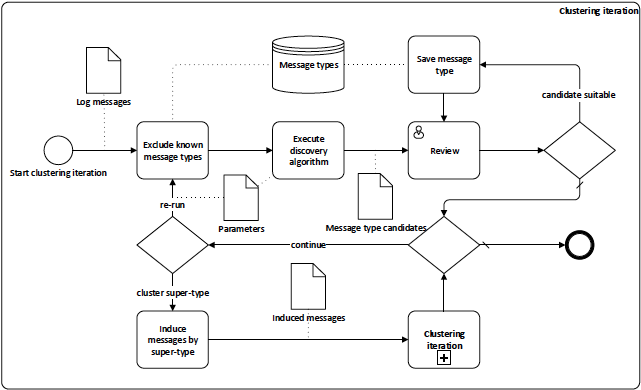
\includegraphics[width=\textwidth]{images/RURC.png} 	
 \end{minipage}
  \caption{Recursive User-Reviewed Clustering, obr. prevzaný z~\parencite{Tovarnak2017}}
  \label{fig:rurc}
\end{figure}


\section{Extended Nagappan-Vouk algoritmus}
\label{sec:eng}
RURC definuje všeobecné princípy analýzy logovacích súborov, avšak nešpecifikuje algoritmus, ktorý má byť použitý na clustrovanie správ.
Z~nedostatkov zmienených v~predchádzajúcej kapitole ale vyplýva, že žiaden algoritmus okrem LogCluster sa nehodí na použitie v~RURC.
\par RNDr. Daniel Tovarňák preto vyvinul algoritmus Extended Na\-gappan-Vouk určený pre použitie v~RURC, ktorý bude spĺnať všetky požiadavky RURC a zároveň bude jednoduchšie nastaviteľný ako LogCluster. Algoritmus produkuje parsovacie vzory vo formáte, ktorý popisuje parameter ako \emph{\%\{m,n\}} $\%\{m,n\}$. Podobne ako pri LogClustri to označuje \emph{m} až \emph{n} za sebou idúcich tokenov. Napr. parsovací vzor \emph{Software caused \%\{1,3\}} zachytí správu, ktorá obsahuje text \emph{Software caused} nasledovaný 1 až 3 slovami oddelenými medzerou. \newpage \par Postup algoritmu:

\begin{enumerate}
 \item Správy sa rozdelia na tokeny na základe užívateľom zadaných oddeľovačov slov.
 \item Algoritmus vybuduje frekvenčnú tabuľku rovnako ako pri klasickom Nagappan-Vouk algoritme. Rozdiel je však v~tom, že~algoritmus si ukladá aj pozície rozdeľovačov slov.
 \item Pre každú správu si vo frekvenčnej tabuľke vyhľadáme frekvencie všetkých tokenov správy. Rozdiel oproti Nagappan-Vouk algoritmu je ten, že hraničnú frekvenciu určíme metódou q-per\-centilu poďla užívateľom zadanej vstupnej hodnoty. Podľa toho označíme tokeny ako statickú časť alebo wildcard.
 \item Použitím heuristiky algoritmus skúsi odhaliť prekrývajúce sa clustre a v~prípade, že také clustre existujú, pripojí špecifickejší cluster k~viac všeobecnému.
 \item Algoritmus deteguje po sebe idúce sekvencie wildcard v~doposiaľ nájdených vzoroch a ak je to možné, tieto sekvencie spojí a~vytvorí
 vzor s~dolnou a hornou hranicou spojených tokenov.
\end{enumerate}

\subsection{Data mining}
\label{sec:data-mining}
Ako sme spomenuli v~sekcii \ref{sec:eng}, Extended Nagappan-Vouk produkuje parametre vzoru vo formáte \emph{\%\{m,n\}}. Výsledný parsovací vzor je teda kompaktný a užívateľsky čitateľný.  Tento formát vieme ďalej jednoduchou úpravou previesť na regulárny výraz používaný štandardnými knižnicami.
\par Po odhalení všetkých parsovacích vzorov väčšinou príde na rad data mining, tzn. pre každú logovaciu správu extrahujeme parametre jej parsovacieho vzoru. To vykonáme nájdením jej parsovacieho vzoru a vrátením zachytených skupín regulárneho výrazu. Triviálny, ale často používaný postup je iterovať cez všetky vzory až kým sa nenájde zhoda. V~najhoršom prípade to znamená prejsť celú množinu vzorov. Takýto prístup je ale neefektívny a môže spôsobovať výkonnostné problémy.
\par Kvôli odstráneniu vyššie zmienených problémov, RNDr. Daniel Tovarňák v~\parencite{regextrie} navrhol stromovú štruktúru Regex Trie - REtrie a~algoritmus, ktorý v~danej štuktúre nájde príslušný parsovací vzor so~zložitosťou $\mathcal{O}(t)$, kde $t$ je počet tokenov v~správe.
\par REtrie akceptuje parsovacie vzory vo formáte YAML súboru:

\begin{figure}[h]
\centering
\begin{minipage}{\textwidth}
\lstset{columns=flexible,breaklines=true,breakatwhitespace=true, showstringspaces=false}
\begin{lstlisting}
regexps:
  INT: [integer, '[0-9]+']
  STRING: [string, '[!-~]+']
  
patterns:
  default:
    pattern1:'Generating %{INT:var1} bit RSA key'
  ssh:
   pattern1:'Illegal user %{STRING:var1} from %{STRING:var2}'
\end{lstlisting} 		
\end{minipage} 
\end{figure}

Pod kľúčom regexps je zoradený zoznam typov regulárnych výrazov. Každý takýto typ sa skladá z~mena, dátového typu a samotného regulárneho výrazu. Kľúč patterns obsahuje parsovacie vzory, ktoré sú združené pod ľubovoľným identifikátorom skupiny vzorov. Parameter parsovacieho vzoru sa potom skladá z~odkazu na typ regulárneho výrazu a mena. Pri hľadaní vhodného typu sa postupuje zhora nadol a použije sa prvý vhodný typ, ktorý sa nájde. Preto je dôležité poradie, v~akom sú dané typy uvedené.  Aby sme mohli ťažiť z~tohto prístupu, výsledný systém musí vedieť zvládnuť konverziu medzi prezentovanými formátmi parsovacích vzorov.
\chapter{Vyhodnotenie Extended Nagappan-Vouk}
Navrhnutý algoritmus adresuje nedostatky už existujúch algoritmov a odstraňuje ich, ale aby bol skutočne použiteľný je potrebné, aby dosahoval  všeobecne presné výsledky a zvládal pracovať aj s vačším množstvom dát. 

\par Ďalej nás bude zaujímať, či vieme ešte viac spresniť jeho výsledky predspracovaním logovacích správ a ako takýto preprocesing ovplyvní výkonnosť algoritmu. Preto budeme skúmať tieto otázky:

\begin{enumerate}
  \item Aká je presnosť algoritmu Extended Nagappan-Vouk na reálnych dátach ?
  \item Ako rýchlo beží algoritmus na netriviálne veľkej množine vstupných správ ?
  \item Vieme zlepšiť presnosť algoritmu predspracovaním vstupných správ ? Ovplyvní to výkonnosť algoritmu ?
\end{enumerate}

Ako základ pre naše vyhodnotenie sme použili štúdiu \parencite{he2016}. Autori v nej nazbierali dáta z piatich produkčných systémov. Tieto dáta manuálne spracovali a vytvorili tzv. golden standard, čiže ideálne rozdelenie správ na clustre. Voči tomuto rozdeleniu potom počítame hodnotu štatistiky F-measure na výsledkoch algoritmu \parencite{goldenstandard}. My sme ďalej pre každý takýto dataset určili hodnoty oddeľovačov slov a dáta sme detailnejšie očistili.

\subsection{Presnosť Extendedd Nagappan-Vouk}
Ako môžme vidieť na obrázku \ref{fig:chart-precision-eng}, algoritmus pre všetky hodnoty Q-Percentilu dosahuje vysoké hodnoty F-Measure. Výnimkou je len dataset BGL, pre ktorý je hodnota F-Measure globálne nížšia. Avšak pri správnom nastavení aj na tomto datasete vieme dosiahnuť uspokojivej presnosti.

	\begin{figure}[htbp]
	 \centering
	 \begin{minipage}[b]{\linewidth} 
	 	\centering	
	 	\begin{tikzpicture}
		\begin{axis}[
	    xlabel = Q-Percentil,
	    ylabel = {F-Measure},
	    legend pos=outer north east
	]
	\addplot [
	    domain=1:100, 
	    mark=x,
	    color=red,
	]
	coordinates {(5,0.0023) (15, 0.0283)  (25,0.0463) (50, 0.1956) (75, 0.7993) (99, 0.4149)};
	\addlegendentry{BGL};
	
	\addplot [
	    domain=1:100, 
	    mark=x,
	    color=blue,
	]
	coordinates {(5,0.9756) (15, 0.9777)  (25,0.9862) (50, 0.9861) (75, 0.9856) (99, 0.9851)};
	\addlegendentry{HPC};
	
	\addplot [
	    domain=1:100, 
	    mark=x,
	    color=green,
	]
	coordinates {(5,0.8111) (15, 0.8220)  (25,0.8528) (50, 0.8547) (75, 0.8547) (99, 0.8547)};
	\addlegendentry{Proxifier};
	
	\addplot [
	    domain=1:100, 
	    mark=x,
	    color=orange,
	]
	coordinates {(5,0.1229) (15, 0.5650)  (25,0.7709) (50, 0.9713) (75, 0.9981) (99, 1.0000)};
	\addlegendentry{SOSP};
	
	\addplot [
	    domain=1:100, 
	    mark=x,
	    color=orange,
	]
	coordinates {(5,0.9903) (15,0.9991)  (25,0.9999) (50, 0.9992) (75, 0.9993) (99, 0.9271)};
	\addlegendentry{Zookeeper};
	 
		\end{axis}
	\end{tikzpicture}
 	\caption{Presnosť algoritmu Extended Nagappan-Vouk}
 	\label{fig:chart-precision-eng}
 \end{minipage}
\end{figure} 


\subsection{Výkonnosť Extendedd Nagappan-Vouk}
Uznávame, že dané datasety o mohutnosti 2000 záznamov nie sú dostačujúce na vyvodenie záveru, ale poskytujú základný prehľad o výkonnosti algoritmu. Keď namerané čísla porovnáme s výsledkami z \parencite{he2016} vidíme, že Extended Nagappan-Vouk pracuje pomalšie ako SLCT alebo IPLoM, ale radovo sú časy behu rovnaké. Je potrebné si všimnúť koreláciu medzi F-Measure a dĺžkou behu algoritmu. Čím je F-Measure vyššie a analýza je presnejšia, tým sa skracuje čas potrebný na spracovanie daného datasetu.

	\begin{figure}[htbp]
	 \centering
	 \begin{minipage}[b]{\linewidth} 
	 	\centering	
	 	\begin{tikzpicture}
		\begin{axis}[
	    xlabel = Q-Percentil,
	    ylabel = {Čas(s)},
	    legend pos=outer north east
	]
	\addplot [
	    domain=1:100, 
	    mark=x,
	    color=red,
	]
	coordinates {(5,14.624) (15, 15.761)  (25,16.479) (50, 9.827) (75, 0.992) (99, 0.709)};
	\addlegendentry{BGL};
	
	\addplot [
	    domain=1:100, 
	    mark=x,
	    color=blue,
	]
	coordinates {(5,0.356) (15, 0.362)  (25,0.342) (50, 0.344) (75, 0.375) (99, 0.348)};
	\addlegendentry{HPC};
	
	\addplot [
	    domain=1:100, 
	    mark=x,
	    color=green,
	]
	coordinates {(5,4.232) (15, 3.895)  (25,0.814) (50, 0.492) (75,0.575) (99, 0.552)};
	\addlegendentry{Proxifier};
	
	\addplot [
	    domain=1:100, 
	    mark=x,
	    color=orange,
	]
	coordinates {(5,12.197) (15, 4.427)  (25,3.604) (50, 0.473) (75, 0.557) (99, 0.503)};
	\addlegendentry{SOSP};
	
	\addplot [
	    domain=1:100, 
	    mark=x,
	    color=orange,
	]
	coordinates {(5,0.565) (15,0.404)  (25,0.463) (50, 0.9992) (75, 0.399) (99, 0.406)};
	\addlegendentry{Zookeeper};
	 
		\end{axis}
	\end{tikzpicture}
 	\caption{Dĺžka behu algoritmu}
 	\label{fig:chart-precision-eng}
 \end{minipage}
\end{figure} 

\subsection{Spresnenie algoritmu predspracovaním}
Zistili sme, že správne odhaliť parsovacie vzory zo správ, ktoré obsahujú parametre typu ip adresa alebo email môže byť náročné, kvôli potrebe správne nastaviť hodnotu oddeľovačov slov tak, aby boli správne rozpoznané ako jeden parameter. 
\par Chceme teda overiť, či dodatočné predspracovanie správ a nahradenie týchto parametrov ich zahešovanou hodnotou, zmenší závislosť na správnom nastavení oddeľovačov slov a zvýši presnosť.

\par Empirickou metódou sme určili zoznam kandidátov na takúto zámenu. Sú to tieto parametre:

\begin{enumerate}
  \item Url
  \item Email
  \item Hostname
  \item Ip adresa
  \item ISO časová známka
\end{enumerate}

Pred samotnou analýzou teda prejdeme všetky správy a každý výskyt jedného z vymenovaných parametrov nahradíme jeho zahešovanou hodnotou. Pri behu algoritmu Nagappan-Vouk teda nedôjde k rozdelenie podľa oddeľovača slov. 
\par Porovnaním výsledkov sme zistili, že nami prezentované riešenie neviedlo k zlepšeniu presnosti parsovacích vzorov. Priemer F-Measure pôvodného algoritmu je 0.81 pričom priemer verzie s predspracovaním je len 0.78. Čísla za jednotlivé datasety ukazujú, že v prípadoch, kde pôvodný algoritmus dosiahol nízku presnosť, upravená verzia nebola schopná túto presnosť výrazne prekonať. V datasetoch s vysokou presnosťou nami upravený algoritmus len kopíruje pôvodnú verziu a pre dataset Zookeeper dokonca zhoršuje priemernú presnosť. 
\par Tieto merania sú ale špecifické tým, že parameter oddeľovačov slov je nastavený podľa znalosti domény daného datasetu a preto pôvodná verzia produkuje veľmi presné výsledky. Ďalej sme zistili, že takéto predspracovanie výkonnosť algoritmu ovplyvňuje len nepatrne.
\chapter{Analýza požiadaviek systému}

Hlavnou úlohou navrhovaného systému je umožniť užívateľovi pohodlne pracovať na odhaľovaní parsovacích vzorov použitím Recursive User-Reviewed Clustering cyklu a algoritmu Extended Nagappan-Vouk. Užívateľské rozhranie musí byť prívetivé a informovať používateľa o~prípadných chybách počas analýzy logovacích správ.

\section{Užívateľské akcie - prípady užitia}

Systém automaticky predpokladá, že užívateľ pri prístupe má v~pláne začat analyzovať logovacie správy. Užívateľ je preto presmerovaný na záložku Miner do stavu začatia novej analýzy. V~tomto stave môže užívateľ zadať zdroj dát, z~ktorého budú pochádzať data analyzované v~ďalšom kroku, alebo tento krok preskočí. Následne môže ako zdroj vstupných dát vybrať logovací súbor alebo použiť nespracované logovacie správy, ktoré sú v~systéme uložené. Dostupné su aj nastavenia algoritmu, ktoré sú špecifické pre nasledovný beh analýzy. Užívateľovi sú potom prezentované nájdené parsovacie vzory, ktoré sa buď môže rozhodnúť potvrdiť alebo s~nimi ďalej pracovať. Uživateľ si ďalej môže nájdené vzory prehliadnuť, zobraziť správy ktoré k~nemu patria, poprípade daný vzor odstrániť. Nájdené vzory sa dajú filtrovať podľa zdroja správ a vyexportovať. Dané prípady užitia sú prezentované na obr. \ref{fig:use-cases}, ktorý je nasledovaný detailnejším popisom.

\clearpage

\begin{figure}[htbp]
 \centering 
 \begin{minipage}{0.9\linewidth}
 	\centering
 	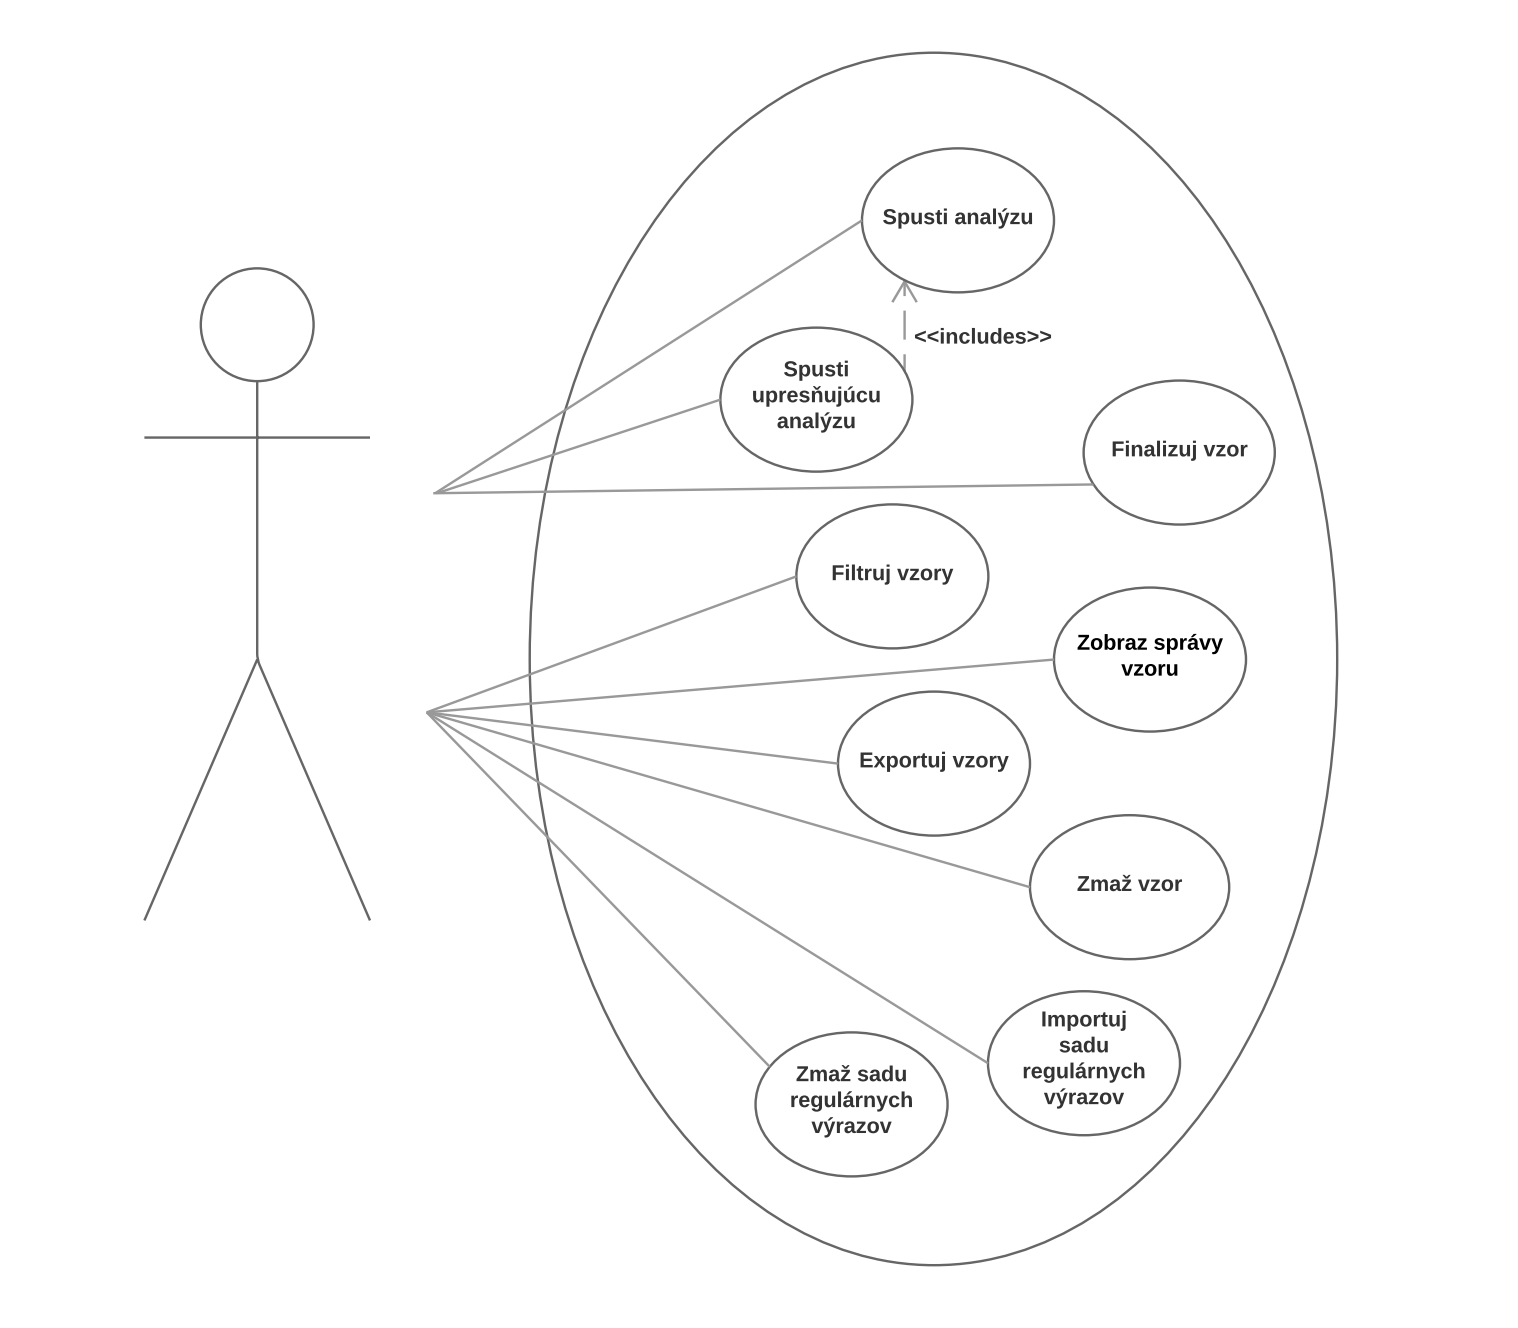
\includegraphics[width=\textwidth]{images/thesis-use-cases.png}	
 \end{minipage}
  \caption{Prípady užitia}
  \label{fig:use-cases}
\end{figure}

\begin{enumerate}
  \item Ako užívateľ zadám vstupný súbor a spustím analýzu
  \begin{enumerate}
  	\item Po zobrazení užívateľského rozhrania môžem zadať zdroj dát pre nasledujúcu analýzu alebo môžem tento krok preskočiť
  	\item Pred spustením môžem meniť hodnotu percentilu a oddeľovačov slov
  	\item V každom momente môžem začať novú analýzu
  \end{enumerate}
  \item Ako užívateľ ktorý už spustil prvotnú analýzu, viem označiť podmnožinu nájdených vzorov a pustiť nad nimi spredňujúcu analýzu
  \item Ako užívateľ ktorý už spustil prvotnú analýzu, vyberiem nájdený vzor a finalizujem ho
  \item Ako užívateľ viem filtrovať medzi nájdenými vzormi podľa zdroja dát
  \item Ako užívateľ viem zobraziť správy, ktoré prislúchajú k danému vzoru
  \item Ako užívateľ viem zmazať nájdený vzor
  \item Ako užívateľ viem exportovať nájdené vzory
  \begin{enumerate}
  	\item Pred exportom si vyberiem sadu regulárnych výrazov, pomocou ktorých sa nájdený vzor prevedie do formátu REtrie.
  \end{enumerate}
  \item Ako užívateľ viem importovať sadu regulárnych výrazov pre export
  \item Ako užívateľ viem zmazať sadu regulárnych výrazov pre export
  \begin{enumerate}
  	\item Ak je daná sada rôzna od defaultnej, ktorá nejde zmazať zo systému
  \end{enumerate}
\end{enumerate}

\section{Komponenty systému}
Po preskúmaní požiadaviek sme dospeli k~záveru, že systém vieme ďalej rozdeliť do týchto kategógií:

\begin{enumerate}
  \item Task queue
  \item Webový backend
  \item Úložisko dát
  \item Užívateľské rozhranie
\end{enumerate}

\subsection{Užívateľské rozhranie}
Užívateľské rozhranie musí byť intuitívne a poskytovať dobrú podporu pre asynchrónne operácie, ktoré bude spúšťať. RURC proces definovaný v~\ref{sec:rurc} môže byť v~budúcnosti ešte rozšíreny, preto je zároveň dôležité aby sa užívateľské rozhranie dalo jednoducho rozšíriť a zdrojový kód udržovať.

\subsection{Webové api}
Backend bude prijímať a spracovávať požiadavky od klienta. Musí vedieť persistovať data, spúštať dlhotrvajúce úlohy na task queue a poskytovať klientovi možnosť zistiť status bežiacej úlohy. Mala by byť použitá dobre známa technológia, ktorá sa dobre integruje a umožnuje rýchly vývoj.

\subsection{Task queue}
Je zodpovedná za beh dlhotrvajúcich operácií. Dôležitá podmienka je by stabilita, výkonnosť a schopnosť zotaviť sa z~chyby. Je podstatné aby po výskyte chyby v~jednom behu úlohy, nebola ovplyvnená schopnosť prijímať ďalšie. Je tu zároveň požiadavka na možnosť dotazovať sa na stav bežiacej úlohy.

\subsection{Úložisko dát}
Dáta s~ktorými sa v~aplikácii pracuje sú jednoducho štrukturované z~relačného pohľadu. Naviac veľkú časť dát tvoria medzivýsledky, ktoré potrebujeme vedieť rýchlo spracovať a uložiť, ale po krátkom čase už nebudú a zo systému budú zmazané. Preto vyvstáva otázka, či sa má použiť tradičná relačná databáza alebo niektorá z~NoSQL databázi. 

\section{Technologické riešenie}

Extended Nagappan-Vouk algoritmus aj RURC cyklus sú dostupné pod slobodnou softvérovou licenciou. Preto aby výsledný systém bol ľahko nasaditeľný a dostupný, všetky technológie a nástroje použité na implementáciu a beh systému by mali byť pod slobodnou licenciou.

\subsection{Programovací jazyk}
Ako programovací jazyk systému sme po úvahe zvolili Python. Python bol vybraný, pretože už je používany v~existujúcich systémoch ÚVT, bol použitý pri referenčnej implementácii spomínaných algoritmov a dobre sa hodí pre použitie v~našom systéme. Python je rozširený a populárny dynamický typovany jazyk, ktorý patrí medzi základnú sadu programov nainštalovaných na väčšine Linuxových distribúcií. Medzi jeho prednosti patria široká škála voľne dostupných knižníc a jednoduchá správa závislostí, napr. použitím balíčkovacieho správcu pip. 

\subsection{Task queue}
Užívateľ si v~klientskej časti navolí parametre a klient pomocou http volania API spustí algoritmus hľadania parsovacích vzorov.
Dĺžka behu spustenej analýzy je silne závislá od počtu vstupných logovacích správ, ale skoro vždy je to časovo náročná operácia a klientská aplikácia by nemala čakať na response až na jej koniec. Preto je potrebné zvoliť riešenie, ktoré túto analýzu spustí na pozadí a ponúka nám možnosť získať výsledky neskôr. Task queue je systém pre paralelné vykonávanie úloh neblokujúcim spôsobom. Task queue pre svoje fungovanie využíva tieto komponenty :

\begin{enumerate}
  \item Broker, prostredník ktorý drží zadané úlohy.
  \item Producent, funkcia ktorá vytvára úlohy a posiela ich na brokera na neskoršie spracovanie.
  \item Konzument, vezme úlohy z~brokera a vykoná ich. Neformálne si konzumenta môžme predstaviť ako jedno vlákno, ktoré čaka na spustenie úlohy.
\end{enumerate}

Ako implementáciu task queue sme vybrali celery, v~súčasnej dobe asi najpoužívanejšie riešenie. Celery je dobre zdokomentované riešenie, ktoré je oproti ostatným variantám komplikovanejšie ale vyniká vo výkone a stabilite. Ako broker sa odporúča využiť RabbitMQ alebo Redis. Vybrali sme Redis, pre jeho možné využitie ako úložisko dát, ako je spomenúté v~\ref{sec:store}.

\subsection{Webový backend}
Pri výbere technológie pre webový backend sme brali do úvahy podporu technológie pre prácu s~celery a následne aj formu akou bude vytvorené užívateľské rozhranie. Rozhodovali sme sa medzi dvoma najzámejšími frameworkami pre python, konk. medzi frameworkami Django a Flask. Django je viac robustné, poskytuje programátorovi väčšiu podporu ale aj väčšie obmedzenia. Flask na druhej strane je jednoduchý framework, ktorý necháva programátorovi väčšiu voľnosť. Oba frameworky podporujú pohodlnú prácu s~celery. Nakoniec sme vybrali Django kvôli dobrej osobnej skúsenosti.

\subsection{Úložisko dát}
\label{sec:store}
Pre ukladanie dát sme sa rozhodli použiť kombináciu relačnej databázy PostgreSQL a in-memory databáze Redis. PostgreSQL je open source databáza, ktorá plne implementuje štandard ANSI SQL a spĺňa vysoké nároky na konzistenciu dát a výkon súčasne. Hoci je PostreSQL  rozsiahly systém z~množstvom nastavení pre ladenie výkonu, je veľmi ľahko nainštalovateľná a už v~základnom nastavení poskytuje dobrú výkonnosť. Navyše framework Django odporúča pri výbere databázy použiť práve PostgreSQL, čo považujeme za výhodu. Redis už v~infraštuktúre máme použitý ako broker pre celery. Mimo to je Redis super rýchle in-memory úložisko typu kľúč hodnota. Poskytuje sadu datových typov, ktorá je postačujúca na uloženie medzivýsledkov a asynchrónne ukladanie dát na disk.
Vo výsledku teda použijeme Redis pre uloženie všetkých neštrukturovaných dát a medzivýsledkov a PostgreSQL prácu so štukturovanými datami. To nám umožnuje dosiahnuť vysoký výkon v~prípade potreby.

\subsection{Užívateľské rozhranie}
Pretože Django poskytuje pomerne dobré templatovacie možnosti rozhodli sme sa túto možnosť využiť ako základ rozhrania. Ale na dosiahnutie interaktivity a asynchrónnosti je nutné použiť javascript. Vybrali sme preto knižnicu jQuery, ktorá sa ľahko integruje a pracuje dobre v~kombinácií s~Djangom. Týmito technológiami bol vytvorený funkčný prototyp, ktorý odhalil určité nedostatky. Pre naimplementovanie zobrazovania výsledných parsovacích vzorov bolo nutné použiť stromovú štruktúru, v~ktorej sme potrebovali pridávať a odoberať uzly na užívateľom zvolenenom mieste v~strome. Práca s~týmto stromom bola s~knižnicou jQuery síce možná, ale obslužný kód bol zbytočne komplikovaný a zle udržovateľný. Preto sme sa rozhodli túto kombináciu nahradiť čisto javascriptovým riešením. Bola zvolená knižnica Angular 2, ktorá je zameraná na vývoj interaktívnych aplikácií, umožňuje krátky vývojový proces a má veľkú sadu vývojárskych nástrojov.
Na štýlovanie užívateľského rozhrania sme použili Bootstrap. Jedná sa o~momentálne najpoužívanejšie riešenie pre tvorbu moderných a responzívnych webov. To umožnilo, že výsledné rozhranie je z~veľkej miery responzívne, aj keď nepredpokladáme jeho časté využitie na mobilných zariadeniach.

\begin{figure}[htbp]
 \centering 
 \begin{minipage}{0.95\linewidth}
 	\centering
 	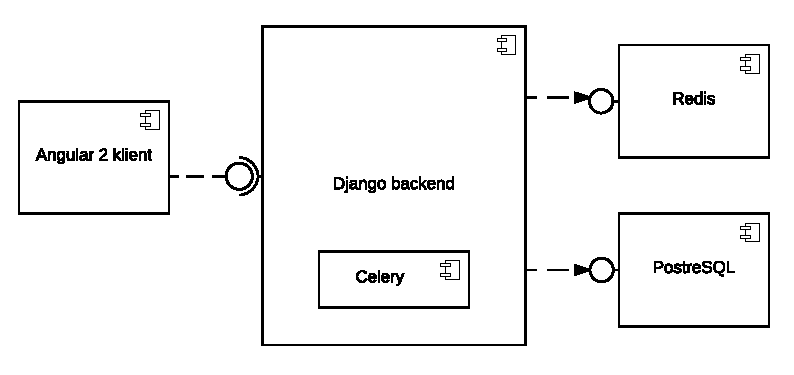
\includegraphics[width=\textwidth]{Images/thesis-component-diagram.pdf}	
 \end{minipage}
  \caption{Komponenty aplikácie }
  \label{fig:components}
\end{figure}

\section{Implementácia systému}
Štruktúru zdrojových kódov sme rozhodli rozdeliť na 3 časti. Servrová časť obsahuje zdrojové kódy v~pythone pre backend a producentov úloh pre celery. Klientska čast zapuzdruje užívateľské rozhranie v~Angular 2 a nástroje potrebné na vývoj a preklad zdrojových kódov. V~inštalačnej časti sú skripty ktoré plne automatizujú nasadenie aplikácie na linuxový server.
\chapter{Serverová časť}
Hlavnou funkcionalitou tejto časti je obslúžiť požiadavky prichádzajúce ako http volania, spracovať ich a vrátiť výsledok vo formáte JSON. Backend sa teda priamo nestará o obslúženie užívateľských akcií a ani o routovanie, ale len odpovedá na volania od klienta. V REST API vystavujeme tieto metódy:

 \begin{minipage}{0.9\linewidth}
 	\centering
 	\missingfigure[figheight=10cm]{tabulka rest api}
 	%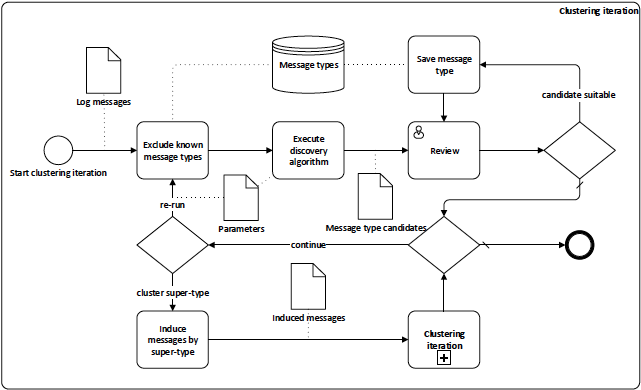
\includegraphics[width=\textwidth]{images/RURC.png} 	
 \end{minipage}
 

Pri implementácii sme sa intenzívne spoliehali na framework Django.
\par Django obsahuje veľké množstvo modulov, z ktorých sme v našej práci síce využili len malú podmnožinu, ktorá nám ale zásadne zjednodušila celú implementáciu. Funkcionalita je rozdelená do samostatných súborov alebo modulov pre jednoduchý a prehľadný kód.

\subsection{Django ORM}
Pre prístup k dátam z databázy je v celej aplikácii použité objektovo-relačné mapovanie zakomponované priamo v Djangu.
\par Využitie Django ORM vo väčšine prípadov vývojára úplne odprostí od potreby implementovať DAL -- Data Access Layer, čiže vrstvu pre prístup k dátam, ako je obvyklé napr. v jazykoch Java alebo C\#. Django ORM používa potomkov triedy \emph{django.db.models.Model}, ďalej nazývaných ako modely, na zadefinovanie štruktúry dát a pôsobí ako jediný prístupový bod k dátam. Každý model reprezentuje tabuľku v databáze a jeho objekt tohto typu jeden riadok v databáze. 

\begin{figure}[htbp]
\centering
\begin{minipage}{0.9\textwidth}
\lstset{tabsize=4,columns=flexible,breaklines=true,breakatwhitespace=true, showstringspaces=false}
\begin{lstlisting}
class Source(models.Model):
    source = models.CharField(max_length=255, blank=False, db_index=True)
    version = models.CharField(max_length=50)

    class Meta:
        unique_together = ('source', 'version')
\end{lstlisting} 		
\end{minipage} 
\caption{Databázový model typu Source}
\label{fig:static-analysis}
\end{figure}

\subsection{Django migrations}
Na vytvorenie databázovej schémy používame Django migrations. 
\par Použitím Django migrations vývojári nemusia písať ddl scripty a modelujú schémy vytváraním tried v jazyku Python. Prvotná schéma je vygenerovaná automaticky, každá ďalšia zmena kódu spôsobí vygenerovanie novej migrácie, ktorá je následne aplikovaná na databázové tabuľky. Tento spôsob sa ukázal ako veľmi nápomocný v deployment scriptoch, kde jednoducho spustíme migráciu príkazom \emph{python manage.py migrate} a na vytvorenie schémy nepotrebujeme dodatočného sql klienta. Zároveň týmto spôsobom vieme do aplikácie vložiť aj iniciálne dáta.

\subsection{Implementácia Extended Nagappan-Vouk}
Implementácia sa snaží byť čo najrýchlejšia, preto používame knižnicu \emph{multiprocessing}. Väčšina vykonávaných metód najprv rozdelí problém na menšie časti, spočíta výsledok podproblému v novom procese a následne problém spojí. 
\par Implementácia začína predspracovaním, v ktorom pre každú správu hľadáme sekvenčným prechodom cez už uložené parsovacie vzory ten správny. Ak nejaký existuje, daná správa je z ďalšieho spracovania vylúčená. Uznávame, že táto operácia nie je veľmi efektívna, ako už bolo zmienené v \ref{sec:data-mining} a s narastajúcim počtom uložených správ značne zhorší celkový čas spracovania, preto môže byť implementácia tejto operácie v budúcnosti jednoducho zameniteľná za riešenie založené na REtrie. 
\par Ďalej nasleduje samotný beh algoritmu, ktorého výsledky sú uložené do Redisu. Za návratoú hodnotu je použitý objekt, ktorý obsahuje štatistiku vytvorenú z týchto výsledkov a textovú reprezentáciu parsovacích vzorov.

\begin{figure}[htbp]
 \centering 
 \begin{minipage}{0.95\linewidth}
 	\centering
 	\missingfigure[figheight=10cm]{diagram komponent}
 	%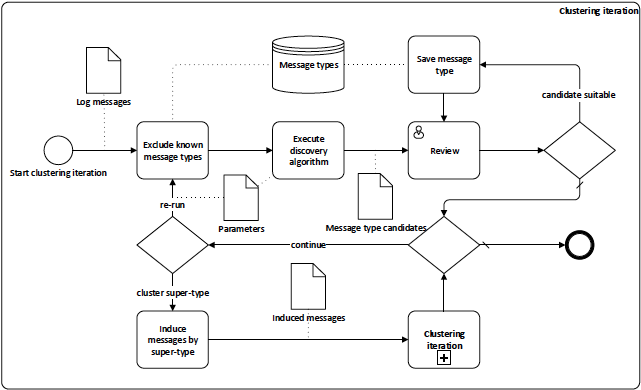
\includegraphics[width=\textwidth]{images/RURC.png} 	
 \end{minipage}
  \caption{ERD diagram vzorov}
  \label{fig:erd-patterns}
\end{figure}

\subsection{Prevod medzi formátmi parsovacích vzorov}
\label{sec:format-transformation}

Pri prevode medzi týmito formátmi potrebujeme mať vopred známu sadu typov regulárnych výrazov, voči ktorým budeme konverziu prevádzať. Je žiadúce, aby táto sada nebola konštantná pre všetky parsovacie vzory, ale aby bolo možné ju zadať pre vybrané parsovacie vzory. Z tohto dôvodu nie je transformácia medzi formátmi prevádzaná pri uložení parsovacieho vzoru, ale je vykonaná on demand pre zadanú sadu typov algoritmom \ref{fig:pattern-transformation}.

\begin{figure}[htbp]
\centering
\begin{minipage}{0.9\textwidth}
\lstset{tabsize=4,columns=flexible,breaklines=true,breakatwhitespace=true, showstringspaces=false}
\begin{lstlisting}
def transform_pattern_to_regex(pattern, pattern_lines, regex_types):
    types_tab = build_pattern_types_tab(pattern, pattern_lines, regex_types)

    transformed_patterns = {}
    pattern_idx = 0
    for line_key, types in types_tab.items():

        idx = 0
        replacements = []
        replacement = ''
        for words_in_groups in line_key.split():
            replacement = ''
            for words_in_group in words_in_groups:
                replacement.append('%{{{name}:var{idx}}}'.format(name=types[idx], idx=idx))
                idx += idx
            replacements.append(replacement)
            
        transformed_patterns['pattern' + pattern_idx] = replace_groups_text(pattern, replacements)

    return transformed_patterns


def build_pattern_types_tab(pattern, pattern_lines, regex_types):
    pattern_types = {}

    for line in pattern_lines:
        pattern_match = pattern.match(line)
        types = []
        keys = []
        pattern_groups = pattern_match.groups()
        for pattern_group in pattern_groups:
            words = pattern_group.split()
            for word in words:
                types.append(find_first_suitable_regex_type(word, regex_types))
            keys.append(str(len(words)))
        line_key = ','.join(keys)
        update_types(pattern_types, line_key, types)

    return pattern_types
\end{lstlisting} 		
\end{minipage} 
\caption{Databázovy model typu Source}
\label{fig:pattern-transformation}
\end{figure}

Hlavný rozdiel medzi popisovanými formátmi je ten, že pokým nativný formát algoritmu Extended Naggap-Vouk skracuje výskyt viacerých parametrov v rade, REtrie formát tento zápis nepozná. Preto vo výsledku z jedného parsovacieho vzoru môže vzniknúť až 

\begin{align*}
\prod_{group \in groups} group.upper\_bound - group.lower\_bound
\end{align*}

nových vzorov. Ďalší rozdiel je neprítomnosť typu parametra v pôvodnom formáte.

\chapter{Klientska časť}
Táto časť poskytuje užívateľské rozhranie, naviguje užívateľa v~rámci aplikácie, reaguje na jeho akcie a komunikuje s~vystaveným rozhraním serverovej časti aplikácie.
\par Klienstka časť je naimplementovaná použitím frameworku Angular 2. Nejedná sa o~tzv. single page, ako je to bežné pri~aplikáciách napísaných v~tomto frameworku, ale je rozdelená na tri stránky, kde si každá drží svoj interný stav. Sú to stranký Miner, Mined Patterns a~Regex Groups. Stránka Miner slúži na samotné odhaľovanie parsovacích vzorov, zatiaľ čo Stránky Mined Patterns a Regex Groups slúžia na prácu s~finalizovanými parsovacími vzormi, resp. sadami typov regulárnych výrazov určených pre transformáciu vzorov.


\section{Angular 2}
Angular 2 je relatívne nový komponentovo-orientovaný JavaScriptový framework, ktorý odstraňuje nedostatky pôvodnej verzie. Aplikácie sa v~Angular 2 píšu buď v~TypeScripte, alebo vo verziách \mbox{ECMAScript}~5 resp. 6. Ani jeden variant zatiaľ nie je plne podporovaný dnešnými prehliadačmi, preto je nutná transkompilácia. My sme použili TypeScript, nadstavbu JavaScriptu, ktorý zavádza statické typovanie a~prvky objektovo-orientovaného programovania ako typy, triedy, moduly a~pod., čo považujeme za veľkú výhodu. Základné stavebné prvky sú:

\begin{enumerate}
 \item Modul -- zpuzdruje funkcionalitu, ktorá vykonáva jednu úlohu. Funguje podobne ako OSGi modul, kde modul vidí len komponenty definované v~samotnom module a komponenty, ktoré modul explicitne importuje. Zároveň modul špecifikuje, ktoré komponenty budú viditeľné zvonku balíčka.
 \item Komponent -- základný prvok aplikácie. Definuje aplikačnú logiku a interaguje so šablónou cez rozhranie vlastností a metód. Potrebná konfigurácia komponentu je zabezpečená cez metadáta.
 \item Šablóna -- html stránka obohatená o~značky z~jazyka Angular. Definuje, ako bude zobrazený komponent. Zároveň obsahuje značkovanie pre prepojenie dát, ktoré určuje, ako sú vymieňané dáta medzi komponentom a šablónou. V~predošlej verzii Angularu sa vždy jednalo o~obojsmerné prepojenie, čo spôsobovalo výkonnostné problémy. Vo verzii 2 si vieme toto prepojenie zašpecifikovať a vyhnúť sa tak týmto problémom.
 \item Servisná služba -- trieda, ktorá obsahuje funkcie na vykonanie špecifických úloh potrebných aplikáciou.
 \item Dependency injection -- spôsob založený na rovnomennom návr\-hovom vzore, ktorým Angular poskytuje servisným službám a~komponentom závislosti.
\end{enumerate}

\subsection{Podporné nástroje}
Aplikácie písané v~Angular 2 sú závislé na knižniciach tretích strán, ako aj na knižniciach samotného Angularu.
\par Na správu týchto závislostí používame všeobecne známy Node.js a~jeho balíčkovací systém npm, zatiaľ čo na správu samotného kódu používame Webpack, jednoduchý balíčkovač zdrojových kódov. Webpack ponúka široké možnosti ako zdrojové kódy upraviť pred výsledným zabalením do archívu, a zároveň možnosť vystaviť tieto kódy v~rámci vývojového servera, čo sme pri vývoji vo veľkej miere využívali. V~našom systéme Webpack pred výsledným zabalením zdrojové kódy minimalizuje a prevedie optimalizácie.
\par Oba tieto nástroje sme ovládali a nastavovali cez nástroj Angular CLI, ktorý umožnuje vygenerovať si projekt už obsahujúci najčastejšiu konfiguráciu.


\subsection{Miner}
Na začiatku je možné určiť aplikáciu, z~ktorej analyzované správy pochádzajú, a jej verziu, ako môžeme vidieť na obr. \ref{fig:miner-source}. Ďalej môžeme určiť, či chceme analyzovať správy z~logovacieho súboru, ktorý nahrajeme, alebo použijeme správy, ktoré už sú v~systéme nahrané a neboli zatiaľ finálne analyzované.

\begin{figure}[htbp]
 \centering 
 \begin{minipage}{0.95\linewidth}
 	\centering
 	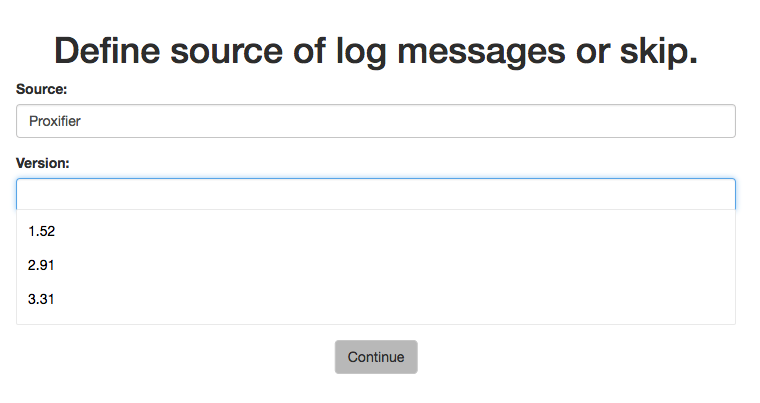
\includegraphics[width=\textwidth]{Images/thesis-miner-source.png}
 \end{minipage}
  \caption{Špecifikovanie zdrojovej aplikácie pre potreby analýzy. \mbox{Vstupné} polia sú umiestnené pod sebou, ako reakcia na šírku okna v~responzívnom dizajne.}
  \label{fig:miner-source}
\end{figure}

Po tomto kroku máme pred sebou rozhranie, ktorým budeme upravovať a spúšťať analýzu.
\par Po upresnení oddeľovačov a q-percentilu užívateľ spustí analýzu. Po obdržaní výsledkov je užívateľovi prezentovaná tabuľka, ktorej hlavnú časť tvoria navrhované parsovacie vzory. V~tabuľke napravo je~tlačidlo, ktorým užívateľ daný parsovací vzor potvrdí ako finálny. Pre~potreby spresňujúcej analýzy je pri každom vzore vľavo checkbox. Pri~označení ľubovoľného počtu navrhovaných vzorov a následnej analýze sú ako vstupné správy brané len tie, ktoré prislúchali k~označeným vzorom. Výsledky spresňujúcej analýzy sú vložené do~tabuľky tak, že novo navrhované parsovacie vzory sú pripojené ako potomkovia vzoru, z~ktorého vznikli, a vytvárajú tak stromovú štruktúru. Tento proces vieme opakovať, až kým nefinalizujeme všetky parsovacie vzory, alebo sa môžeme rozhodnúť pre začatie novej analýzy.

\begin{figure}[htbp]
 \centering 
 \begin{minipage}{0.95\linewidth}
 	\centering
 	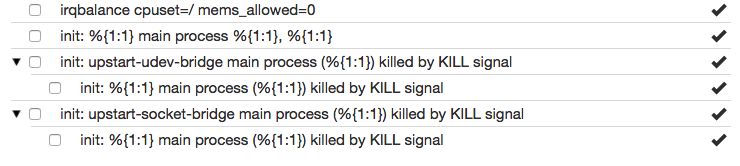
\includegraphics[width=\textwidth]{Images/thesis-miner-analysis.png}
 \end{minipage}
  \caption{Priebeh analýzy logovacích správ.}
  \label{fig:miner-source}
\end{figure}

\subsection{Mined patterns}
Rozhranie prezentuje stránkovací zoznam finalizovaných parsovacích vzorov, ktoré si je možné vyfiltrovať podľa zdrojovej aplikácie a jej verzie, ako vidíme na obrázku \ref{fig:pattern}. Aktuálny vyfiltrovaný zoznam si~užívateľ vie exportovať do formátu REtrie. Zoznam ďalej umožnuje náhľad na správy, ktoré boli vygenerované, použitím vybraného parsovacieho vzoru.

\begin{figure}[htbp]
 \centering 
 \begin{minipage}{0.95\linewidth}
 	\centering
 	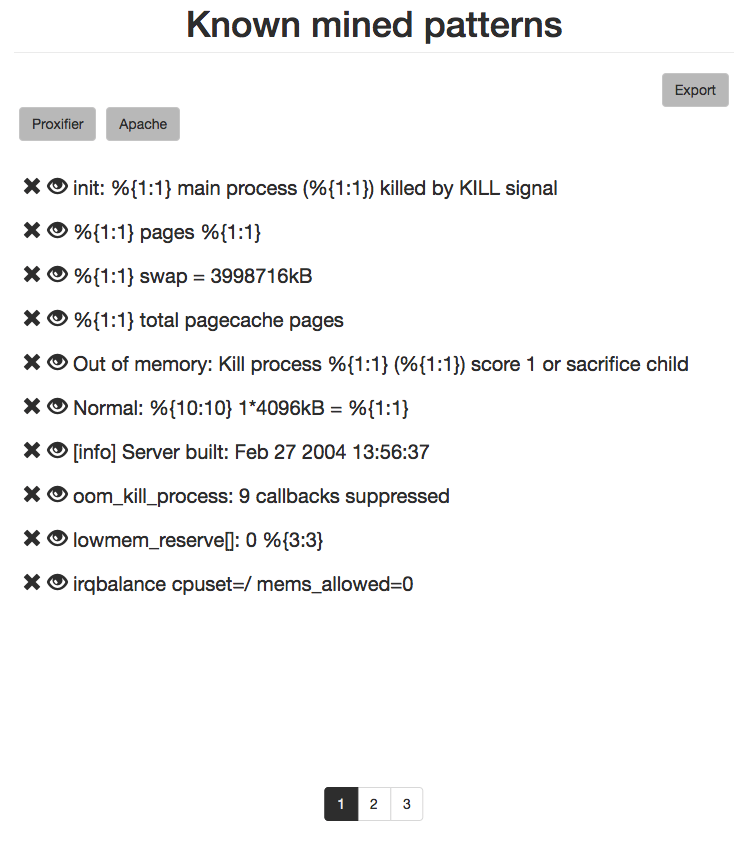
\includegraphics[width=\textwidth]{Images/thesis-pattern.png}
 \end{minipage}
  \caption{Správa uložených parsovacích vzorov.}
  \label{fig:pattern}
\end{figure}

\subsection{Regex Groups}
Zobrazuje zoznam sád typov regulárnych výrazov, ktoré sú v~aplikácií nahrané. V~systéme sme prednastavili základnú sadu, ktorá by mala byť postačujúca pre značnú časť prípadov a táto sada nejde zo systému zmazať. Systém ďalej umožnuje nahrať novú sadu zo súboru vo~formáte:

 \begin{figure}[htbp]
 \centering 
 \begin{minipage}{0.95\linewidth}
 	\centering
 	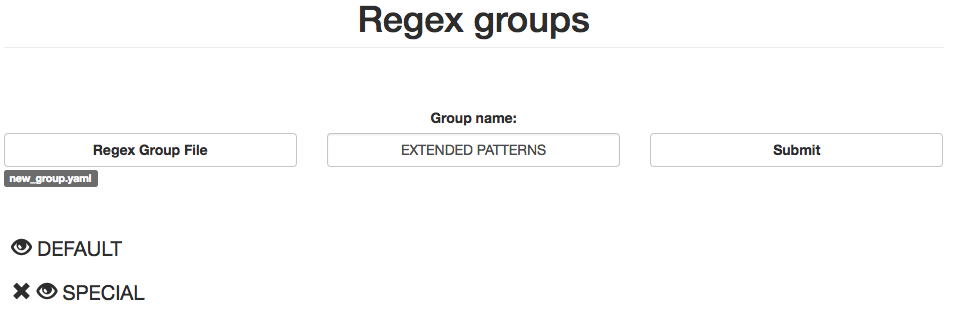
\includegraphics[width=\textwidth]{Images/thesis-groups.png}
 \end{minipage}
  \caption{Importovanie novej skupiny a aktuálny zoznam.}
  \label{fig:groups}
\end{figure}

\chapter{Inštalácia a nasadenie}
Implementovaná aplikácia používa len voľne dostupné knižnice a nástroje, ktoré sú schopné bežat na všetkých majoritných operačných systémoch. Predpokladáme ale, že aplikácia bude hlavne nasadená na linuxový server ako je to bežné. Preto sme vytvorili scripty, ktoré by mali administrátorovi pomôcť automatizovať proces nasadenia na linuxový server RHEL len za použitia nevyhnutne minimálnej konfigurácie. Použili sme pritom python virtuálne prostredie, konzolové nástroje Fabric a Ansible.

\section{Príprava prostredia}
V tejto fáze si aktivujeme python virtuálne prostredie a prostredníctvom pip balíčkovacieho manažéra si nainštalujeme Fabric.
Fabric je nástroj, ktorý nám dovolí písaním python kódu volať služby operačného systému. Týmto spôsobom: 

\begin{enumerate}
  \item Vygenerujeme ssh kľúče
  \item Prihlásime sa na cieľový systém a updatujeme ho
  \item Vytvoríme užívateľa a skupinu pod ktorou bude bežať naša aplikácia
  \item Nahrajeme vygenerované ssh kľúče
  \item Upgradujeme server a nainštalujeme závislosti pre Ansible
\end{enumerate}

\chapter{Záver}
Našou úlohou bolo zoznámiť sa v algoritmom Extended Nagappan-Vouk a jeho použitím pri odhaľovaní parsovacích vzorov v logových súboroch. Ďalej sme mali naimplementovať systém, ktorý umožní užívateľovi pracovať s týmto algoritmom a skúsiť zlepšiť jeho presnosť dodatočným predspracovaním.
\par V úvode sme si najprv predstavili problematiku odhaľovania parsovacích vzorov, algoritmy na ich odhaľovanie a popísali ich nedostatky. Potom sme hlbšie preskúmali samotný algoritmus Extended Nagappan-Vouk a meraním ukázali jeho presnosť. 
\par V priebehu implementácie sme sme nenarazili na žiadne závažnejšie problémy, ktoré by ohrozili výsledok práce. Výsledný systém je plne funkčný a môže byť nasadený v rámci XXX.
\par v budúcnosti XXX.

 \printbibliography

\end{document}
